% C=1 namerno zadržava oznake A=1,0 iz originala, uz indekse 4,5/6,7.
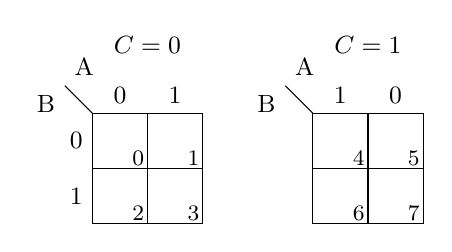
\begin{tikzpicture}[font=\fontsize{9}{10}\selectfont,x=7mm,y=7mm,baseline=(current bounding box.center)]
\draw (0,0) rectangle (2,2) (1,0)--(1,2) (0,1)--(2,1);
\draw (0,2)--(-.5,2.5) node[above right] {A} node[below left] {B};
\node[above] at (.5,2) {0};\node[above] at (1.5,2) {1};
\node[left] at (0,1.5) {0};\node[left] at (0,.5) {1};
\node[above] at (1,2.9) {\(C=0\)};
\foreach \x/\y/\lab in {1/1/0,2/1/1,1/0/2,2/0/3}{
 \node[anchor=south east,inner sep=1pt,font=\fontsize{8}{9.5}\selectfont] at (\x,\y) {\lab};
}
\draw (4,0) rectangle (6,2) (5,0)--(5,2) (4,1)--(6,1);
\draw (4,2)--(3.5,2.5) node[above right] {A} node[below left] {B};
\node[above] at (4.5,2) {1};\node[above] at (5.5,2) {0};
\node[above] at (5,2.9) {\(C=1\)};
\foreach \x/\y/\lab in {5/1/4,6/1/5,5/0/6,6/0/7}{
 \node[anchor=south east,inner sep=1pt,font=\fontsize{8}{9.5}\selectfont] at (\x,\y) {\lab};
}
\end{tikzpicture}
